\documentclass[12pt, a4paper]{article}
\usepackage{graphicx}
\graphicspath{ {./imgs/} }
\usepackage{float}
\usepackage{listings}
\usepackage{color}

\definecolor{codegreen}{rgb}{0,0.6,0}
\definecolor{codegray}{rgb}{0.5,0.5,0.5}
\definecolor{codeorange}{rgb}{1,0.49,0}
\definecolor{backcolour}{rgb}{0.95,0.95,0.96}

\lstset{
  backgroundcolor=\color{backcolour},   
  commentstyle=\color{codegray},
  keywordstyle=\color{codeorange},
  numberstyle=\tiny\color{codegray},
  stringstyle=\color{codegreen},
  basicstyle=\ttfamily\footnotesize,
  breakatwhitespace=false,         
  breaklines=true,                 
  captionpos=b,                    
  keepspaces=true,                 
  numbers=left,                    
  numbersep=5pt,                  
  showspaces=false,                
  showstringspaces=false,
  showtabs=false,                  
  tabsize=2,
  xleftmargin=10pt,
}
\renewcommand{\lstlistingname}{Code}

\counterwithin{figure}{section}

%to write code:
%\begin{lstlisting}[language=java or bash]
%    
%\end{lstlisting}

%to insert an image
%\begin{figure}[H]
%  \centering
%  \includegraphics[scale=0.33]{img.png}
%  \caption{description of the image}
%\end{figure}

\begin{document}
  \title{Web Architectures - Delivery 1}
  \author{Marrocco Simone}
  \maketitle
  \tableofcontents
  \pagebreak

  \section{Section 1 - Modified MiniHTTPD project}
  \subsection{Introduction}
  The objective of this assignment was to modify the MiniHTTPD project given by the professor and adding some code so that the server, when the url starts with \textit{process/}, launches an external process that takes the input from the query parameters and returns an output. In particular, we needed to create the process that reverses the input string and outputs it, made in a new java file.

  \subsection{Modify \textit{TinyHttpdConnection.java}}
  \subsubsection{Inside \textit{run()}}
  In the overriden function \textit{run()} we add the pieces of code written below.

  First, we intercept only the requests that start with \textit{process/}, since there may be files that start with \textit{process} which we do not want to serve in this particular if-case. 

  Inside it, we use different combinations of \textit{String.split()} and controls to ensure that the url is in the form \\\textbf{process/reverse/query\_name=query\_value} and if not we call the function \textit{sendErrorBadRequest}, that sends an error page (its code is explained later), with a specific error message.

  When we are sure to have the correct command and at least one query, we call the function \textit{callExternalProcess} with input the value of the first query param. Notice how, in line 22 of the code below, we split on every non letter characted: in this way, the String \textit{command[1]} will be separated on all values \textbf{=} and \textbf{\&}.

  We finally return the output of the external process with a basic HTTP header.

  \begin{lstlisting}[language=java, caption={Code added inside run()}]
///// old code
if (req.endsWith("/") || req.equals("")) {
  req = req + "index.html";
}
// ASSIGNMENT 1 - Marrocco Simone
if (req.startsWith("process/")) {
    // req should be 'process/reverse?query_name=query_value', otherwise error
    String[] url = req.split("/");
    if (url.length != 2){
        sendErrorBadRequest(ps, req, "Too many page requested. Ask only one command");
        return;
    }
    String[] command = url[1].split("\\?");
    if (!command[0].equals("reverse")){
        sendErrorBadRequest(ps, req, "Command not yet implemented");
        return;
    }
    if (command.length != 2){
        sendErrorBadRequest(ps, req, "No query given");
        return;
    }
    String[] queries = command[1].split("[\\W]");
    if (queries.length < 2){
        sendErrorBadRequest(ps, req, "incorrect or null queries");
        return;
    }
    String query_value = queries[1];
    String output = callExternalProcess(query_value);
    ps.print("HTTP/1.1 200 OK\r\n");
    ps.print("Content-Type: text/html\r\n");
    ps.print("\r\n");
    ps.print(output);
} else
// OPEN REQUESTED FILE AND COPY IT TO CLIENT
///// continue with old code
\end{lstlisting}

  \subsubsection{Extra functions used}

  We also use two functions: the first is simply to send a page with code 400 Bad Request and an error message explaining why the request was bad.

  The second function is used to call the external process and return the output. The function does not deal with \textbf{IOException} errors but leaves the calling function, in this case \textit{run}, to deal with it (as it already does).

  The external process called is a java command with input the \textbf{ReverseString.java} file location and the user input. However, to get the first one we need to use absolute location on our machine: that means not only that the system is not secure, but the server launch would not work in another machine without changing this path. This is caused by the IntelliJ run command, that moves the compiled files to the Tomcat location which is, of course, a totally different path. For the scope of this deliverable, however, it can be ignored: to start the project we just need to change the line 14 of the code below.

  The rest of the code uses the \textbf{ProcessBuilder} class to create the process and get the output.

  \begin{lstlisting}[language=java, caption={functions added to the class TinyHttpdConnection}]
/** error page sent when bad request while processing a /process/ request */
private void sendErrorBadRequest(PrintStream ps, String req, String error_msg) {
    ps.print("HTTP/1.1 400 Bad Request\r\n\r\n");
    ps.println(error_msg);
    ps.println("The wrong URL: "+req);
    System.out.println("400 Bad Request: " + req);
}

/** call the external process that uses another Java file */
protected String callExternalProcess(String input) throws IOException {
    /** the bash command used. Instead of a single String with spaces, we need an array of Strings */
    String[] bash_command = {
            "java",
          "/home/simone/Java/Projects/MiniHTTPD-Marrocco/src/it/unitn/disi/webarch/tinyhttpd/ReverseString.java",
            input
    };

    ProcessBuilder processBuilder = new ProcessBuilder();
    processBuilder.command(bash_command);
    Process process = processBuilder.start();
    BufferedReader bufferedReader = new BufferedReader(new InputStreamReader(process.getInputStream()));
    StringBuilder stringBuilder = new StringBuilder();
    String line = null;
    while ( (line = bufferedReader.readLine()) != null) {
        stringBuilder.append(line);
        stringBuilder.append(System.getProperty("line.separator"));
    }
    String result = stringBuilder.toString();
    return result;
}
\end{lstlisting} 

  \subsection{\textit{ReverseString.java}}
  The external process called is a java command with input this file that takes a String as an argument, reverses it with the \textbf{StringBuilder} class and prints it.

  \begin{lstlisting}[language=java, caption={Class that reverses a string}]
package it.unitn.disi.webarch.tinyhttpd;

public class ReverseString {
    public static void main(String[] a){
        String inputString = a[0];
        if(inputString == null) System.out.println("ERROR: no params given");
        System.out.println(new StringBuilder(inputString).reverse());
    }
}
\end{lstlisting}
  
  \subsection{Results}

  The server is correctly built. Here are some screenshots of the results.

  \begin{figure}[H]
    \centering
    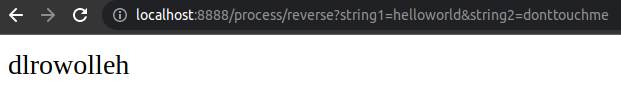
\includegraphics[scale=0.6]{server_ok.png}
    \caption{The server processes correctly the first query parameter. Other ones are ignored}
  \end{figure}

  \begin{figure}[H]
    \centering
    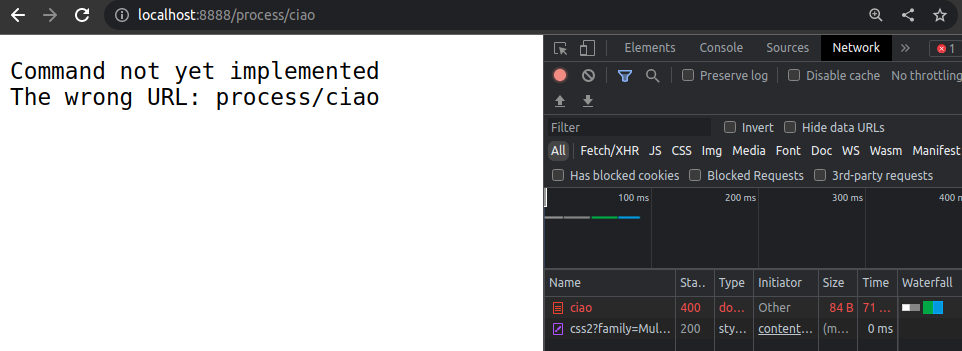
\includegraphics[scale=0.4]{server_no_command.png}
    \caption{If a different command than \textit{reverse} is given, the server returns 400 with an explanation}
  \end{figure}  
  
  \begin{figure}[H]
    \centering
    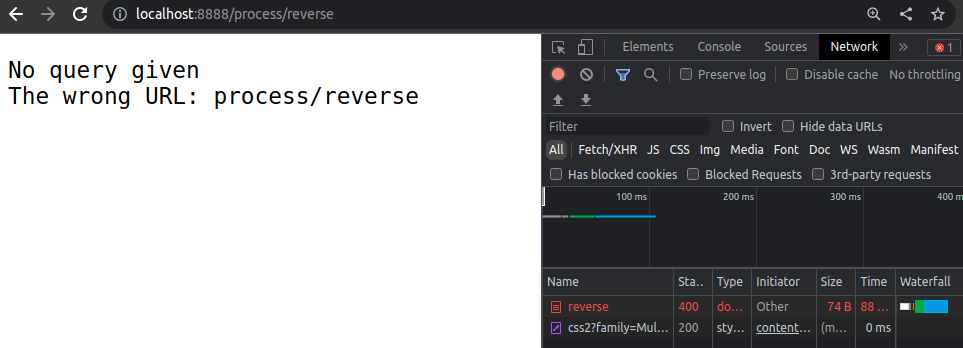
\includegraphics[scale=0.4]{server_no_qeury.png}
    \caption{If there are no query parameters, the server returns 400 with an explanation}
  \end{figure}

  \section{Section 2 - Apache serving a bash file using the java program made before}
  \subsection{Introduction}
  The objective of the second part was to install correctly Apache with Xampp and, inside the cgi-bin folder write a bash file that does the same as the server above: taking input from the query params, calling \textbf{ReverseString.java} to process it and returning the output. This script file would then be calleable from the browser web at the adress \textit{localhost/cgi-bin/file.sh} when Apache is running.

  \subsection{\textit{reverseString.sh}}
  The bash file below takes the query params from the global variable \\\textit{\$QUERY\_STRING} given by Apache, and splits it with the command \\\textbf{\$\{ QUERY\_STRING\#\#\*\=\}}. In particular, this command takes the substring from the last equal sign to the end, so on the contrary of the first assignment this file would not serve only the first query parameter value, but only the last one.

  We can see how here we have the same problem as before on the \textbf{ReverseString.java} file location. We also need to specify the \textbf{\$JAVA\_HOME} location, since Apache is not capable of reading it from our system (or, like this case, use the entire path of the command).

  \begin{lstlisting}[language=bash,caption={file bash used to call ReverseString.java}]
#!/bin/sh
file="/home/simone/Java/Projects/MiniHTTPD-Marrocco/src/it/unitn/disi/webarch/tinyhttpd/ReverseString.java";
query_value=${QUERY_STRING##*=};
output=$(/home/simone/Java/openjdk-19_linux-x64_bin/jdk-19/bin/java $file $query_value);

echo "Content-type: text/plain; charset=iso-8859-1";
echo;
echo "queries: $QUERY_STRING";
echo "query value: $query_value";
echo "output: $output";
\end{lstlisting} 
  
  \subsection{Results}

  The file is correctly executed. Here are some screenshots of the results.

  \begin{figure}[H]
    \centering
    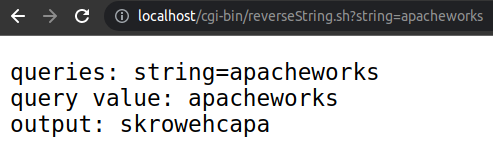
\includegraphics[scale=0.75]{apache_ok.png}
    \caption{The server processes correctly the query parameter}
  \end{figure}

  \begin{figure}[H]
    \centering
    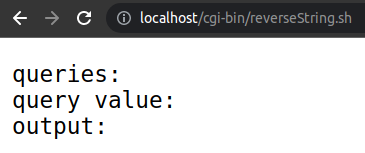
\includegraphics[scale=1]{apache_no_query.png}
    \caption{If there are no query parameters, the server returns an empty string}
  \end{figure} 
\end{document}